\subsection{Community Detection}
An important aspect of social network analysis is the detection of communities within a graph.

\subsubsection{Clustering}
Clustering is one approach to identifying communities within a social network. A cluster within a social network represents a group of people who do not share many interactions with other people outside of their cluster.

\subsubsection{\emph{k}-Cliques}
The term $clique$ is introduced by \citeauthor{luce49} in \cite{luce49} to describe a subgraph which consists of at least three vertices, each of which are fully connected with each other. From a social network perspective, this translates to saying that for each person in the clique, all of their friends  within the clique are friends of each other as well.

A \emph{k}-clique is defined as a clique which has size \emph{k}. A \emph{maximal clique} is a clique to which no more vertices can be added without violating the conditions of a clique, and the maximum clique is a clique within a graph which contains the largest number of vertices.

\begin{figure}[htbp]
\centering
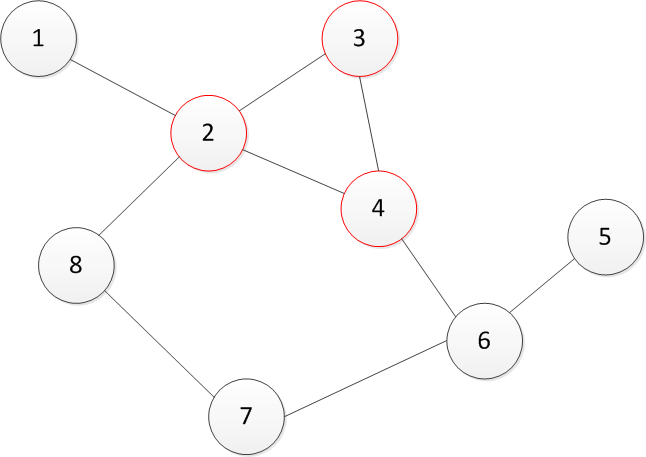
\includegraphics[width=0.7\textwidth]{./img/clique.png}
\caption{Graph highlighting a 3-clique}
\label{fig:clique}
\end{figure}

Figure \ref{fig:clique} shows an example graph highlighting a 3-clique. It has one maximum clique \{2,3,4\} which is highlighted in red, and six other maximal cliques \{1,2\}, \{2,8\}, \{4,6\}, \{5,6\}, \{6,7\}, \{7,8\}.

\begin{figure}
  \centering
  \subfloat[3-clique]{\label{fig:gull}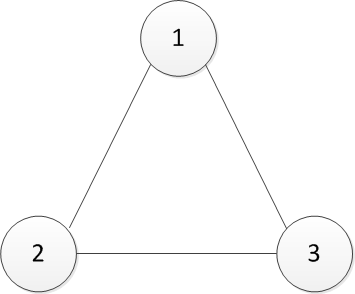
\includegraphics[width=0.3\textwidth]{./img/3-clique}} ~ \subfloat[4-clique]{\label{fig:tiger}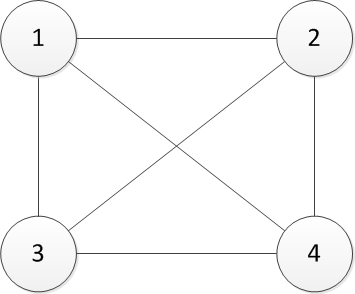
\includegraphics[width=0.3\textwidth]{./img/4-clique}} ~ \subfloat[5-clique]{\label{fig:mouse}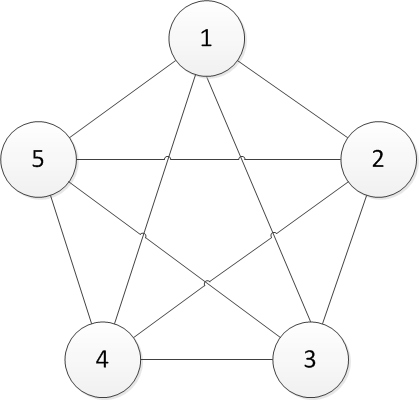
\includegraphics[width=0.3\textwidth]{./img/5-clique}}
  \caption{\emph{k}-cliques}
  \label{fig:cliques}
\end{figure}

Identifying \cite{bomze99}

\subsubsection{\emph{k}-Trusses}

\subsubsection{Clustering Coefficients}
Clustering coefficients provide a way to observe the 
